\def\doctitle{Build the Coupled-Coil Instrument}\def\docsubtitle{A low-voltage pulse and resonance platform}\def\docstrap{the course synthesis, inside the learner boundary}
\def\materialslist{\item 2--4 AA cells in a fused, switched holder
\item Two cardboard bobbins, insulated magnet wire, and a removable ferrite or laminated-iron core
\item Momentary pushbutton, multimeter, ruler, masking tape, and fine sandpaper
\item Cardboard base, insulated jumpers, and cable ties
\item Optional: two LEDs wired antiparallel, each with its own 1 k\(\Omega\) resistor}
\def\prediction{Which change should most increase the receiver indication: aligning the coils, adding the core, or holding DC continuously?}
\def\diagram{\begin{center}
\begin{tikzpicture}[font=\scriptsize,>=Stealth]
  \node[inner sep=0] (plate) {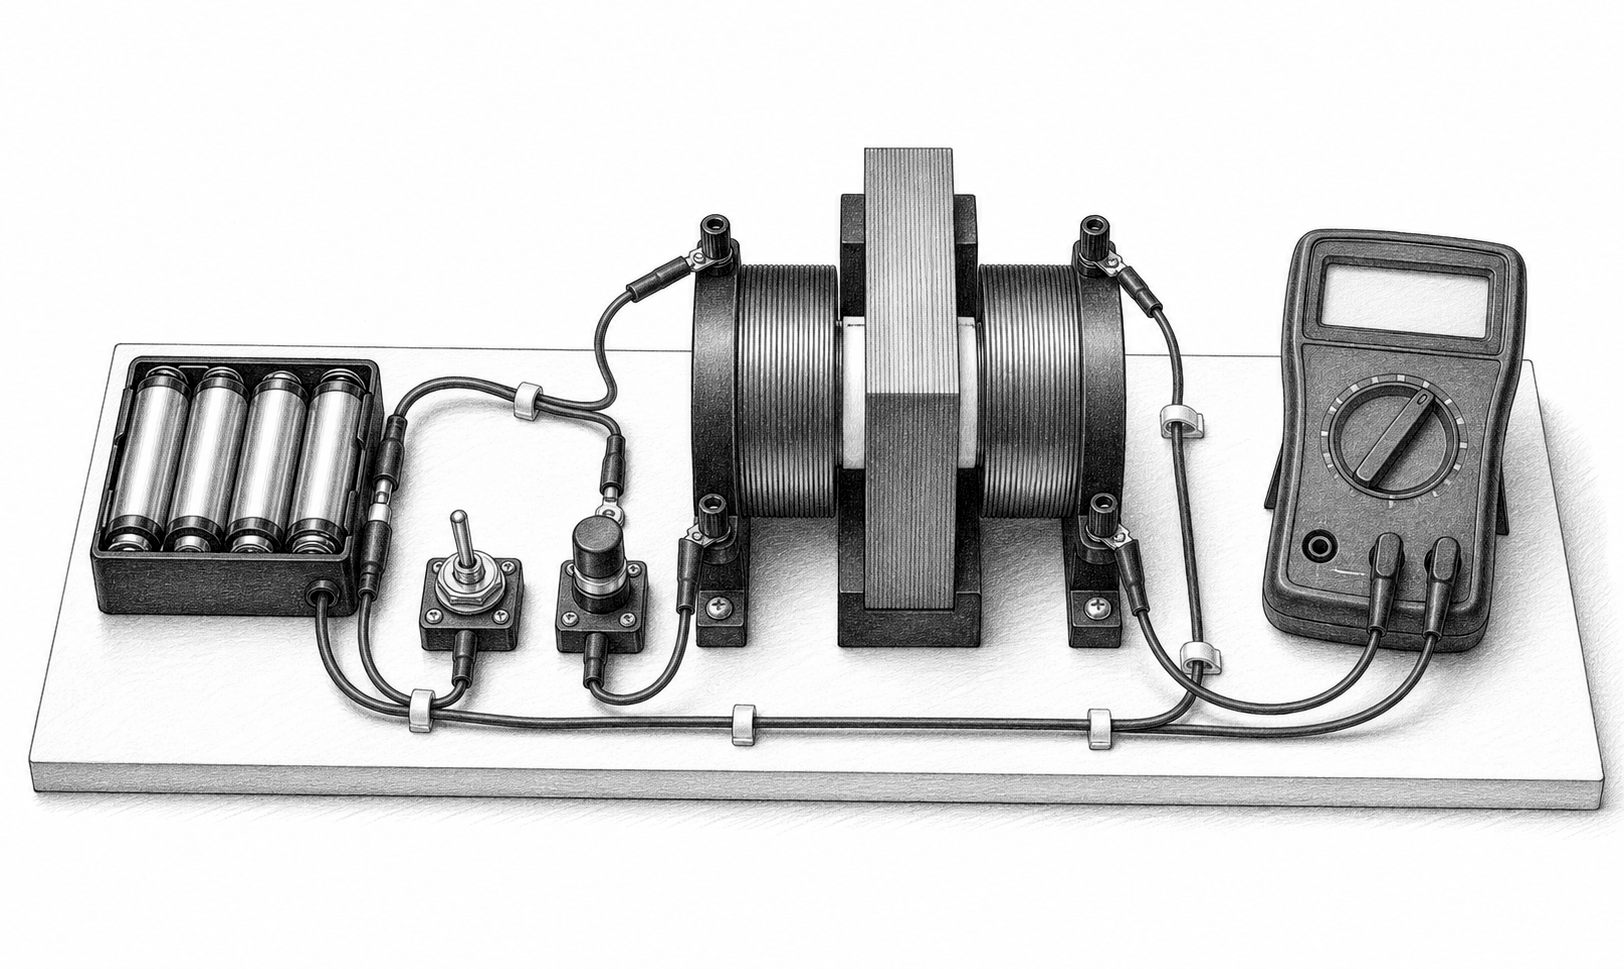
\includegraphics[width=\linewidth]{electricity/chatgpt/build-the-coil/art/coupled-coil-apparatus.png}};
  \node[align=center,fill=white,fill opacity=.9,text opacity=1] at ($(plate.north west)!0.13!(plate.north east)+(0,-1mm)$) {fused holder\\\(4\times\mathrm{AA}\), \(6\,\mathrm{V\,DC}\)};
  \node[align=center,fill=white,fill opacity=.9,text opacity=1] at ($(plate.north west)!0.34!(plate.north east)+(0,-1mm)$) {master\\switch};
  \node[align=center,fill=white,fill opacity=.9,text opacity=1] at ($(plate.north west)!0.42!(plate.north east)+(0,-1mm)$) {momentary\\pushbutton};
  \node[align=center,fill=white,fill opacity=.9,text opacity=1] at ($(plate.north west)!0.50!(plate.north east)+(0,-1mm)$) {primary\\coil};
  \node[align=center,fill=white,fill opacity=.9,text opacity=1] at ($(plate.north west)!0.61!(plate.north east)+(0,-1mm)$) {removable\\core};
  \node[align=center,fill=white,fill opacity=.9,text opacity=1] at ($(plate.north west)!0.70!(plate.north east)+(0,-1mm)$) {secondary\\coil};
  \node[align=center,fill=white,fill opacity=.9,text opacity=1] at ($(plate.north west)!0.89!(plate.north east)+(0,-1mm)$) {meter on\\volts range};
  \draw[->] ($(plate.north west)!0.50!(plate.north east)+(0,-6mm)$) -- ($(plate.north west)!0.49!(plate.north east)+(0,-27mm)$);
  \draw[->] ($(plate.north west)!0.61!(plate.north east)+(0,-6mm)$) -- ($(plate.north west)!0.60!(plate.north east)+(0,-25mm)$);
  \draw[->] ($(plate.north west)!0.70!(plate.north east)+(0,-6mm)$) -- ($(plate.north west)!0.69!(plate.north east)+(0,-27mm)$);
  \draw[<->] ($(plate.south west)!0.48!(plate.south east)+(0,18mm)$) -- node[below,fill=white,inner sep=1pt]{adjustable separation} ($(plate.south west)!0.68!(plate.south east)+(0,18mm)$);
\end{tikzpicture}
\end{center}
\begin{telospanel}{Read the finished instrument before building}
The primary is the only coil connected to the battery. The secondary is an
isolated receiver connected only to the voltmeter or the optional
resistor-limited LED pair. The core slides through both bobbins; it is not an
electrical conductor in either circuit. Every change happens with the master
switch off and the battery holder disconnected.
\end{telospanel}}

\newcommand{\stateplate}{%
\begin{center}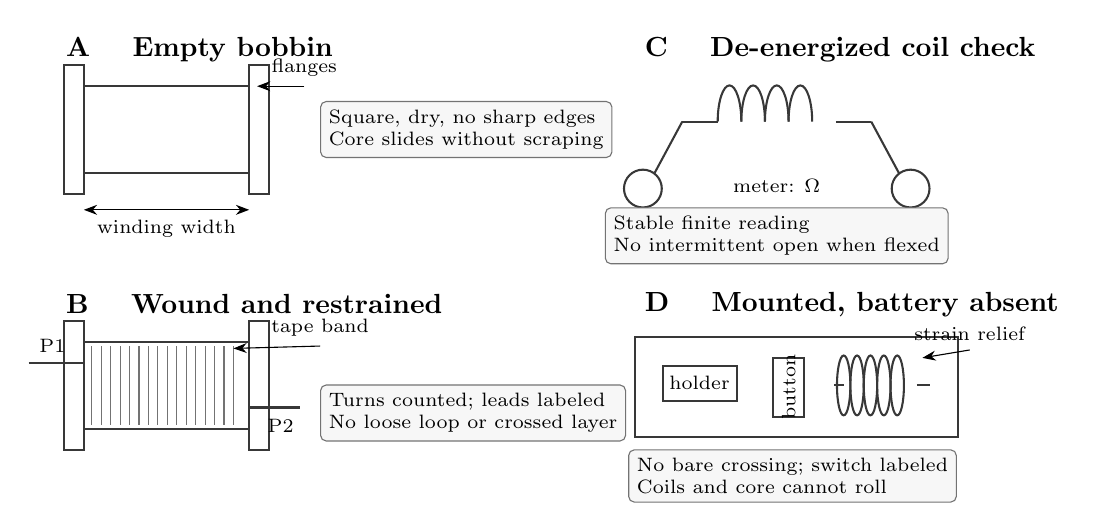
\begin{tikzpicture}[font=\scriptsize,>=Stealth,x=1cm,y=1cm]
\tikzset{sketch/.style={line width=.75pt,draw=black!78},
gate/.style={rounded corners=2pt,draw=black!55,fill=black!3,inner sep=3pt}}
% A: bobbin
\begin{scope}[shift={(0,3.25)}]
\node[anchor=west,font=\bfseries] at (0,1.02) {A \quad Empty bobbin};
\draw[sketch] (.35,-.55) rectangle (2.45,.55);
\draw[sketch] (.1,-.82) rectangle (.35,.82);
\draw[sketch] (2.45,-.82) rectangle (2.7,.82);
\draw[<->] (.35,-1.02)--node[below]{winding width} (2.45,-1.02);
\draw[->] (3.15,.55)--(2.55,.55) node[pos=0,above]{flanges};
\node[gate,align=left,anchor=west] at (3.35,0)
 {Square, dry, no sharp edges\\Core slides without scraping};
\end{scope}
% B: winding
\begin{scope}[shift={(0,0)}]
\node[anchor=west,font=\bfseries] at (0,1.03) {B \quad Wound and restrained};
\draw[sketch] (.35,-.55) rectangle (2.45,.55);
\draw[sketch] (.1,-.82) rectangle (.35,.82);
\draw[sketch] (2.45,-.82) rectangle (2.7,.82);
\foreach \x in {.45,.57,...,2.33}{\draw[black!55] (\x,-.5)--(\x,.5);}
\draw[sketch] (-.35,.28)--(.35,.28);
\draw[sketch] (2.45,-.28)--(3.1,-.28);
\node[above] at (-.05,.3){P1};
\node[below] at (2.85,-.3){P2};
\draw[->] (3.35,.5)--(2.25,.47) node[pos=0,above]{tape band};
\node[gate,align=left,anchor=west] at (3.35,-.35)
 {Turns counted; leads labeled\\No loose loop or crossed layer};
\end{scope}
% C: resistance
\begin{scope}[shift={(7.35,3.25)}]
\node[anchor=west,font=\bfseries] at (0,1.02) {C \quad De-energized coil check};
\draw[sketch] (.6,.1)--(1.05,.1);
\foreach \x in {1.05,1.35,...,2.25}{\draw[sketch] (\x,.1) arc (180:0:.15 and .46);}
\draw[sketch] (2.55,.1)--(3,.1);
\draw[sketch] (.6,.1)--(.25,-.55);
\draw[sketch] (3,.1)--(3.35,-.55);
\draw[sketch] (.1,-.75) circle (.24);
\draw[sketch] (3.5,-.75) circle (.24);
\node at (1.8,-.72){meter: \(\Omega\)};
\node[gate,align=left] at (1.8,-1.35)
 {Stable finite reading\\No intermittent open when flexed};
\end{scope}
% D: mounted, powerless
\begin{scope}[shift={(7.35,0)}]
\node[anchor=west,font=\bfseries] at (0,1.03) {D \quad Mounted, battery absent};
\draw[sketch] (0,-.65) rectangle (4.1,.62);
\draw[sketch] (.35,-.2) rectangle (1.3,.25);
\node at (.82,.03){holder};
\draw[sketch] (1.75,-.4) rectangle (2.15,.35);
\node[rotate=90] at (1.95,-.02){button};
\foreach \x in {2.65,2.82,...,3.5}{\draw[sketch] (\x,0) ellipse (.085 and .38);}
\draw[sketch] (2.53,0)--(2.65,0);
\draw[sketch] (3.58,0)--(3.75,0);
\draw[->] (4.25,.45)--(3.65,.35) node[pos=0,above]{strain relief};
\node[gate,align=left] at (2,-1.15)
 {No bare crossing; switch labeled\\Coils and core cannot roll};
\end{scope}
\end{tikzpicture}\end{center}}

\newcommand{\pulseplate}{%
\begin{center}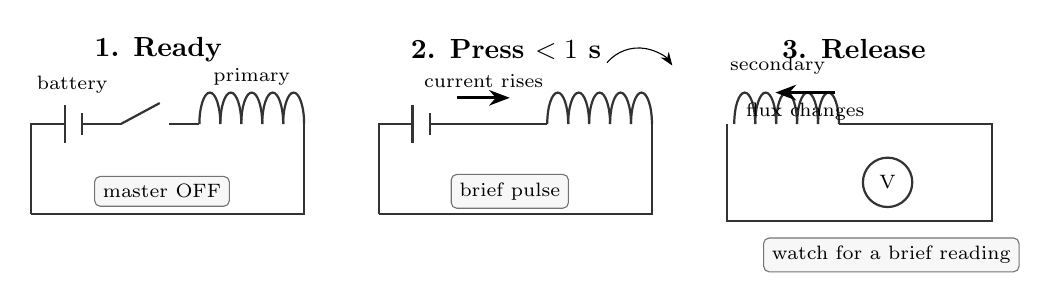
\begin{tikzpicture}[font=\scriptsize,>=Stealth,x=.95cm,y=.95cm]
\tikzset{wire/.style={line width=.8pt,draw=black!80},
off/.style={rounded corners=2pt,draw=black!55,fill=black!3,inner sep=3pt}}
\node[font=\bfseries] at (1.7,2.2){1. Ready};
\draw[wire] (0,0)--(0,1.2)--(.45,1.2);
\draw[wire] (.45,.95)--(.45,1.45);\draw[wire] (.68,1.05)--(.68,1.35);
\draw[wire] (.68,1.2)--(1.2,1.2);
\draw[wire] (1.2,1.2)--(1.72,1.48);
\draw[wire] (1.85,1.2)--(2.25,1.2);
\foreach \x in {2.25,2.53,...,3.37}{\draw[wire] (\x,1.2) arc (180:0:.14 and .42);}
\draw[wire] (3.65,1.2)--(3.65,0)--(0,0);
\node[off] at (1.75,.3){master OFF};
\node at (.55,1.72){battery};
\node at (2.95,1.83){primary};

\begin{scope}[shift={(4.65,0)}]
\node[font=\bfseries] at (1.7,2.2){2. Press \(<1\) s};
\draw[wire] (0,0)--(0,1.2)--(.45,1.2);
\draw[wire] (.45,.95)--(.45,1.45);\draw[wire] (.68,1.05)--(.68,1.35);
\draw[wire] (.68,1.2)--(1.2,1.2);
\draw[wire] (1.2,1.2)--(1.85,1.2)--(2.25,1.2);
\foreach \x in {2.25,2.53,...,3.37}{\draw[wire] (\x,1.2) arc (180:0:.14 and .42);}
\draw[wire] (3.65,1.2)--(3.65,0)--(0,0);
\draw[->,line width=1pt] (1.05,1.55)--(1.75,1.55) node[midway,above]{current rises};
\node[off] at (1.75,.3){brief pulse};
\draw[->] (3.05,2.02) arc (140:35:.55);
\end{scope}

\begin{scope}[shift={(9.3,0)}]
\node[font=\bfseries] at (1.7,2.2){3. Release};
\foreach \x in {.1,.38,...,1.22}{\draw[wire] (\x,1.2) arc (180:0:.14 and .42);}
\draw[wire] (0,1.2)--(0,-.1)--(3.55,-.1)--(3.55,1.2)--(1.5,1.2);
\draw[wire] (2.15,.42) circle (.33);\node at (2.15,.42){V};
\draw[->,line width=1pt] (1.45,1.62)--(.65,1.62) node[midway,below]{flux changes};
\node[off] at (2.2,-.55){watch for a brief reading};
\node at (.68,1.98){secondary};
\end{scope}
\end{tikzpicture}\end{center}}

\newcommand{\acceptancetable}{%
\begin{center}\small
\begin{tabularx}{\linewidth}{@{}p{.18\linewidth}p{.22\linewidth}p{.20\linewidth}L@{}}
\toprule
Gate & Measure & Pass evidence & If it does not pass\\
\midrule
Bobbin & core clearance; winding width & slides freely; edges smooth & reshape or replace before winding\\
Primary & turns; \(R_P\); flex test & count recorded; finite, stable \(R_P\) & expose/clean leads; rewind if open\\
Secondary & turns; \(R_S\); flex test & count recorded; finite, stable \(R_S\) & find broken lead or rewind\\
Mounting & exposed copper; pull test & none; every part restrained & insulate and add strain relief\\
Power path & battery voltage; switch state & expected holder voltage; OFF is open & adult corrects wiring; do not pulse\\
Pulse & peak indication, 3 trials & repeatable response on press/release & use diagnostic path below\\
\bottomrule
\end{tabularx}
\end{center}}

\def\procedure{%
\subsection{Gate 0: freeze the design on paper}
Choose one primary and one secondary bobbin that fit the same removable core.
Plan 100--200 neat turns per coil; use the same turn count first so geometry,
not ratio, is the first variable. Draw the lead names P1/P2 and S1/S2 before
winding.

\begin{predict}
Where could enamelled wire become bare? What prevents a loose turn, a pulled
lead, or a battery lead from crossing another terminal? Point to each control
on the drawing before touching materials.
\end{predict}

\stateplate

\subsection{Gate 1: make and measure each coil}
\begin{enumerate}
\item With the battery holder absent, inspect each bobbin. Round or tape every
edge that could scrape enamel. Measure winding width and core clearance.
\item Leave a 10 cm lead and tape it down as P1. Wind the primary in one
direction, laying turns beside one another. Count aloud in groups of ten and
mark each group on paper. Never wind on a powered circuit.
\item Tape the final layer without hiding the two lead ends. Leave 10 cm for
P2. Repeat for S1/S2 on the second bobbin.
\item The adult removes enamel only from the last 1 cm of each lead. With the
meter on ohms and no battery present, record \(R_P\) and \(R_S\). Gently flex
one lead at a time: the reading must remain finite and stable.
\end{enumerate}

\begin{predict}
If the meter says OL, is the coil a conductor? If it reads nearly zero, what
must be ruled out before connecting cells? Explain why a visual turn count
cannot replace the resistance test.
\end{predict}

\subsection{Gate 2: mount the powerless instrument}
Fasten the holder, master switch, pushbutton, bobbins, and meter leads to the
base. Add strain relief before making electrical joints. Slide the core through
both bobbins and confirm that it can be removed without touching a terminal.
Wire the primary path as holder--fuse--master switch--pushbutton--primary--holder.
Connect the secondary only to the voltmeter. The adult traces both paths with a
finger, then uses continuity mode to verify that OFF is open and a pressed
button conducts only when the master switch is ON.

\begin{predict}
Can current travel from either secondary lead to either primary lead? The
required answer is no continuity. If there is continuity, stop: what contact,
stray strand, or mistaken connection could have joined the isolated circuits?
\end{predict}

\acceptancetable

\subsection{Gate 3: verify one controlled pulse}
\pulseplate
Set the meter to a low DC-voltage range on the secondary. Start with the coils
aligned, touching, and sharing the core. The adult installs 2 AA cells, reads
the holder voltage, and turns the master switch on. The learner presses the
button for less than one second and releases it. Record the largest visible
secondary indication on press and on release. Switch OFF and disconnect the
holder. Repeat three times only after confirming that the coil and holder
remain at room temperature.

\begin{predict}
Why may the meter briefly indicate one sign on press and the other on release?
Why is holding the button down not a stronger induction test? What observation
would make you stop immediately?
\end{predict}

\subsection{Gate 4: change one thing}
Choose exactly one: remove the core, add a measured gap, rotate one coil, or
change the cell count within 2--4 AA cells. Keep turns, meter range, pulse time,
and lead orientation fixed. Make three trials at each setting. Between trials:
master OFF, holder disconnected, touch-check for warmth, then reposition.

\subsection{Diagnostic path: no repeatable indication}
\begin{enumerate}
\item \textbf{Power absent?} Disconnect the coils. Adult verifies holder
voltage, fuse, master switch, and pushbutton continuity. Reconnect only after
the path passes.
\item \textbf{Primary open?} With cells removed, remeasure P1--P2 while gently
flexing leads. OL or jumping values means repair or rewind.
\item \textbf{Receiver open or mis-set?} Remeasure S1--S2, confirm leads are in
the meter COM/V jacks, and confirm volts rather than amps or ohms.
\item \textbf{Coupling weak?} Return to zero gap, coaxial bobbins, and the core
fully inserted. Recheck one brief pulse.
\item \textbf{Instrument too slow?} Reverse the secondary leads and observe
both press and release. A display may miss a short transient; that is a limit
of the measurement, not permission to raise voltage or make sparks.
\end{enumerate}
Stop if a fuse opens twice, a coil warms, insulation is damaged, or any result
is unexplained. Do not bypass the fuse and do not substitute mains, a large
battery, a capacitor, an ignition coil, or a spark gap.}

\def\explanation{This instrument combines current-produced field, changing
flux, mutual induction, and geometry. The secondary responds while primary
current changes---at press and release---not simply because DC exists. Alignment,
small gap, a shared magnetic core, and turn count affect linked flux. The
instrument deliberately does not make sparks and is not a Tesla coil. A
repeatable low-energy pulse and an honest record provide better evidence than
an uncontrolled high-voltage spectacle.}

\def\extension{Make a calibration plot of peak receiver indication versus
separation: 0, 5, 10, 20, and 40 mm, three trials each. Add range bars from the
smallest to largest trial. Then complete this acceptance record:
\begin{center}\small
\begin{tabularx}{\linewidth}{@{}p{.24\linewidth}L@{}}
Primary & turns \rule{1.2cm}{.3pt}\quad \(R_P=\)\rule{1.4cm}{.3pt}\(\Omega\)\\[.8em]
Secondary & turns \rule{1.2cm}{.3pt}\quad \(R_S=\)\rule{1.4cm}{.3pt}\(\Omega\)\\[.8em]
Supply / fuse & \rule{.85\linewidth}{.3pt}\\[.8em]
Baseline geometry & core \rule{1.4cm}{.3pt}\quad gap \rule{1.1cm}{.3pt} mm\\[.8em]
Three baseline peaks & \rule{.85\linewidth}{.3pt}\\[.8em]
Stop checks & no warmth [\enspace]\quad no odor [\enspace]\quad insulation intact [\enspace]\\[.8em]
Adult inspection & initials \rule{1.4cm}{.3pt}\quad date \rule{2.1cm}{.3pt}\\
\end{tabularx}
\end{center}
Photograph or redraw the accepted wiring and label every energy-transfer stage.}
% Telos shared preamble.
%
% Every Telos publication is designed to be printed on a home laser printer,
% one sheet at a time, and carried into a boat or a garage. Two constraints
% follow from that and govern everything below:
%
%   1. Pure monochrome. No value is ever a hue. Emphasis is carried by rule
%      weight, fill, and type, never by color, so a grayscale or black-only
%      printer loses nothing.
%   2. Card density. A "one-pager" is a hard contract: the leaf must fit on a
%      single side of US Letter. The layout is therefore tight by default and
%      the environments below are sized to leave room for a plate.

\documentclass[10pt,letterpaper]{article}

\usepackage[margin=0.55in,includefoot,footskip=0.24in]{geometry}
\usepackage[T1]{fontenc}
\usepackage[utf8]{inputenc}
\usepackage{lmodern}
\usepackage{microtype}
\usepackage{array}
\usepackage{booktabs}
\usepackage{longtable}
\usepackage{tabularx}
\usepackage{enumitem}
\usepackage{needspace}
\usepackage{multicol}
\usepackage{ragged2e}
\usepackage{graphicx}
\usepackage{wrapfig}
\usepackage{xcolor}
\usepackage{fancyhdr}
\usepackage{titlesec}
\usepackage{hyperref}
\usepackage[most]{tcolorbox}
\usepackage{tikz}
\usetikzlibrary{arrows.meta,calc,positioning,shapes.geometric,decorations.pathmorphing,patterns,fadings}

% Semantic names are kept so a document reads intelligibly, but every value is
% black, white, or a neutral gray that survives a black-only print driver.
\definecolor{telosink}{gray}{0}
\definecolor{telospaper}{gray}{1}
\definecolor{telosrule}{gray}{0.35}
\definecolor{telosfill}{gray}{0.90}
\definecolor{telosdeep}{gray}{0.72}
\definecolor{telosmute}{gray}{0.45}

\hypersetup{hidelinks,pdfborder={0 0 0}}

% Keep an unchanged source byte-reproducible across rebuilds: no build-clock
% creation date and no random trailer ID.
\pdfinfoomitdate=1
\pdftrailerid{}

\setlength{\parindent}{0pt}
\setlength{\parskip}{0.42em}
\setlength{\tabcolsep}{4pt}
\setlength{\columnsep}{1.1em}
\renewcommand{\arraystretch}{1.18}
\setlist[itemize]{leftmargin=1.15em,itemsep=0.12em,topsep=0.2em,parsep=0pt}
\setlist[enumerate]{leftmargin=1.5em,itemsep=0.18em,topsep=0.2em,parsep=0pt}
\setlist[description]{leftmargin=0pt,itemsep=0.16em,topsep=0.2em,parsep=0pt,
  font=\normalfont\bfseries}

% ---------------------------------------------------------------------------
% Document identity. Each leaf declares these before \begin{document} so the
% running head, the colophon, and the PDF metadata all agree.
% ---------------------------------------------------------------------------
\newcommand{\TelosProject}{Telos}
\newcommand{\TelosDocTitle}{}
\newcommand{\TelosDocSubtitle}{}
\newcommand{\TelosRevision}{}

\newcommand{\telosmeta}[4]{%
  \renewcommand{\TelosProject}{#1}%
  \renewcommand{\TelosDocTitle}{#2}%
  \renewcommand{\TelosDocSubtitle}{#3}%
  \renewcommand{\TelosRevision}{#4}%
  \hypersetup{pdftitle={#2},pdfsubject={#3; version #4},
    pdfkeywords={Telos, version #4},pdfauthor={Telos}}%
}

\pagestyle{fancy}
\fancyhf{}
\renewcommand{\headrulewidth}{0pt}
\renewcommand{\footrulewidth}{0.4pt}
\fancyfoot[L]{\footnotesize\textsc{\TelosProject}}
\fancyfoot[C]{\footnotesize\TelosDocTitle}
\fancyfoot[R]{\footnotesize\thepage}

% The first page of a one-pager carries the masthead instead of a running foot,
% so its footer is the compact provenance line.
\fancypagestyle{telosfirst}{%
  \fancyhf{}%
  \renewcommand{\headrulewidth}{0pt}%
  \renewcommand{\footrulewidth}{0.4pt}%
  \fancyfoot[L]{\footnotesize\textsc{\TelosProject}}%
  \fancyfoot[C]{\footnotesize\TelosRevision}%
  \fancyfoot[R]{\footnotesize\thepage}%
}

% ---------------------------------------------------------------------------
% Masthead. A heavy rule, the title, a light subtitle, a thin rule. The
% optional argument is a right-aligned tag (a species' scientific name, a
% lesson number) that sits on the title's baseline.
% ---------------------------------------------------------------------------
\newcommand{\telosmasthead}[1][]{%
  \thispagestyle{telosfirst}%
  \begingroup
  \setlength{\parskip}{0pt}%
  \noindent\rule{\linewidth}{1.6pt}\par
  \vspace{0.30em}
  \noindent
  \begin{minipage}[b]{0.66\linewidth}
    \raggedright{\LARGE\bfseries\TelosDocTitle}
  \end{minipage}%
  \hfill
  \begin{minipage}[b]{0.32\linewidth}
    \raggedleft{\small\itshape #1}
  \end{minipage}\par
  \vspace{0.18em}
  \noindent{\small\TelosDocSubtitle}\par
  \vspace{0.28em}
  \noindent\rule{\linewidth}{0.4pt}\par
  \endgroup
  \vspace{0.35em}
}

% ---------------------------------------------------------------------------
% Headings. Compact, small-caps, rule-anchored — a card has no room for the
% article class's default vertical air.
% ---------------------------------------------------------------------------
\titleformat{\section}{\normalfont\large\bfseries}{}{0pt}{}[\vspace{-0.55em}\rule{\linewidth}{0.4pt}]
\titlespacing*{\section}{0pt}{0.85em}{0.35em}
\titleformat{\subsection}{\normalfont\normalsize\bfseries}{}{0pt}{}
\titlespacing*{\subsection}{0pt}{0.6em}{0.2em}
\titleformat{\subsubsection}{\normalfont\small\bfseries\scshape}{}{0pt}{}
\titlespacing*{\subsubsection}{0pt}{0.45em}{0.12em}

% A short run-in heading for card interiors that must not consume a full line.
\newcommand{\telosrubric}[1]{\textbf{#1}\enspace}

% Cross-reference helper. Every Telos project is a set of loose printed sheets,
% so a reference names the sheet rather than a page number.
\newcommand{\sheetref}[1]{\textit{see the \textbf{#1} sheet}}

% Which decision, ADR or sheet governs the paragraph you are reading. A reader
% who disagrees with an instruction should be able to find the reasoning behind
% it rather than having to take it on trust.
\newcommand{\governedby}[1]{{\footnotesize\textsc{governed by #1}}}

% ---------------------------------------------------------------------------
% Quantities. siunitx is not in this TeX Live split, and the guides need only a
% fixed thin space and upright units, so define that directly rather than take
% a package dependency the documented install would not satisfy.
%   \qty{9}{kV}  ->  9 kV        \unitof{kV}  ->  kV
% ---------------------------------------------------------------------------
\newcommand{\unitof}[1]{\ensuremath{\mathrm{#1}}}
\newcommand{\qty}[2]{#1\,\unitof{#2}}
\newcommand{\numrange}[2]{#1\,--\,#2}
\newcommand{\qtyrange}[3]{#1\,--\,#2\,\unitof{#3}}
% Inches and feet appear constantly in the fishing guide; keep one spelling.
\newcommand{\inch}[1]{#1\,in}
\newcommand{\feet}[1]{#1\,ft}

% ---------------------------------------------------------------------------
% Cards and boxes.
% ---------------------------------------------------------------------------

% Titled card with a hairline frame. The default card for facts a reader looks
% up rather than reads through.
\newtcolorbox{teloscard}[1]{
  enhanced, breakable,
  colback=telospaper, colframe=telosink, colbacktitle=telospaper,
  coltitle=telosink,
  boxrule=0.5pt, sharp corners,
  left=6pt, right=6pt, top=4pt, bottom=4pt,
  toptitle=3pt, bottomtitle=3pt, titlerule=0.4pt,
  before skip=6pt, after skip=6pt,
  title={#1}, fonttitle=\small\bfseries
}

% Untitled left-ruled block: hierarchy without a redundant label.
\newtcolorbox{telosframe}{
  enhanced, breakable,
  colback=telospaper, frame hidden, boxrule=0pt, sharp corners,
  borderline west={1.3pt}{0pt}{telosink},
  left=8pt, right=2pt, top=3pt, bottom=3pt,
  before skip=6pt, after skip=6pt
}

% Filled emphasis panel — the "read this first" block. The 10% fill stays
% legible under a cheap laser toner curve and still reads as distinct.
\newtcolorbox{telospanel}[1]{
  enhanced, breakable,
  colback=telosfill, colframe=telosink, colbacktitle=telosfill,
  coltitle=telosink,
  boxrule=0.5pt, sharp corners,
  left=6pt, right=6pt, top=4pt, bottom=4pt,
  toptitle=3pt, bottomtitle=3pt, titlerule=0.4pt,
  before skip=6pt, after skip=6pt,
  title={#1}, fonttitle=\small\bfseries
}

% Hazard block. Deliberately the heaviest object on any page: a 1.4pt frame
% plus a solid title bar. Nothing else in Telos is allowed to look like this,
% so a reader skimming a lesson cannot mistake it for ordinary emphasis.
\newtcolorbox{teloshazard}[1]{
  enhanced, breakable,
  colback=telospaper, colframe=telosink,
  colbacktitle=telosink, coltitle=telospaper,
  boxrule=1.4pt, sharp corners,
  left=6pt, right=6pt, top=5pt, bottom=5pt,
  toptitle=3pt, bottomtitle=3pt,
  before skip=8pt, after skip=8pt,
  title={\MakeUppercase{#1}}, fonttitle=\small\bfseries
}

% A stop-and-check gate. Used before anything destructive, and before anything
% that would be expensive to discover later. Shared by every project that has
% a procedure someone could get hurt following carelessly.
\newtcolorbox{gate}[1]{
  enhanced, breakable,
  colback=telospaper, colframe=telosink,
  boxrule=1.0pt, sharp corners,
  left=6pt, right=6pt, top=4pt, bottom=4pt,
  toptitle=3pt, bottomtitle=3pt, titlerule=0.4pt,
  before skip=7pt, after skip=7pt,
  colbacktitle=telospaper, coltitle=telosink,
  title={\MakeUppercase{#1}}, fonttitle=\small\bfseries
}

% ---------------------------------------------------------------------------
% Rating dots. A five-step scale that prints identically in black-only: filled
% versus open circles, never a shaded bar.
% ---------------------------------------------------------------------------
\newcommand{\telosdot}{\tikz[baseline=-0.42ex]\fill[telosink] (0,0) circle (0.28ex);}
\newcommand{\telosopendot}{\tikz[baseline=-0.42ex]\draw[telosink,line width=0.28pt] (0,0) circle (0.28ex);}
\makeatletter
\newcounter{telos@rate}
\newcommand{\telosrating}[1]{%
  \begingroup
  \setcounter{telos@rate}{0}%
  \@whilenum\value{telos@rate}<#1\do{\telosdot\kern0.22em\stepcounter{telos@rate}}%
  \@whilenum\value{telos@rate}<5\do{\telosopendot\kern0.22em\stepcounter{telos@rate}}%
  \endgroup
}
\makeatother

% ---------------------------------------------------------------------------
% Tables.
%
% tabularx reads its body by scanning for a literal \end{tabularx}, so it can
% never be wrapped in a \newenvironment. Documents therefore open tabularx and
% longtable directly and take their house style from these column types and the
% booktabs rules. The one exception is the fact strip below, which is built on
% plain tabular precisely so it *can* be an environment.
% ---------------------------------------------------------------------------
\newcolumntype{L}{>{\raggedright\arraybackslash}X}
\newcolumntype{R}{>{\raggedleft\arraybackslash}X}
\newcolumntype{C}{>{\centering\arraybackslash}X}
\newcolumntype{B}{>{\bfseries\raggedright\arraybackslash}X}
\newcolumntype{N}{>{\raggedright\arraybackslash}p{0.16\linewidth}}

% Key/value fact strip. Two flush columns of short lookups; the label column is
% a fixed fraction so a stack of cards aligns across the whole guide.
\newenvironment{telosfacts}[1][0.24]
  {\begingroup\small
   \setlength{\parskip}{0pt}%
   \renewcommand{\arraystretch}{1.25}%
   \begin{tabular}{@{}>{\bfseries\raggedright\arraybackslash}p{\dimexpr#1\linewidth\relax}@{\hspace{0.7em}}>{\raggedright\arraybackslash}p{\dimexpr\linewidth-#1\linewidth-0.7em\relax}@{}}}
  {\end{tabular}\par\endgroup}
\newcommand{\telosfact}[2]{#1 & #2\\}

% ---------------------------------------------------------------------------
% Seasonal / diurnal activity bar.
%
% \telosseasonbar{4,3,2,1,1,2,3,3,4,5,4,3} draws a twelve-cell month strip
% where each value 0-5 is a fill height. Height, not gray value, carries the
% signal, so it is exact under any toner curve; the cell is outlined either way
% so an empty month is still visibly a month.
% ---------------------------------------------------------------------------
\newcommand{\telosseasonlabels}{J,F,M,A,M,J,J,A,S,O,N,D}
\newcommand{\telosseasonbar}[1]{%
  \begingroup
  \begin{tikzpicture}[x=1.25em,y=2.1ex,baseline=0pt]
    \foreach \v [count=\i from 0] in {#1} {
      \draw[telosrule,line width=0.3pt] (\i,0) rectangle (\i+0.86,5);
      \ifnum\v>0
        \fill[telosink] (\i,0) rectangle (\i+0.86,\v);
      \fi
    }
    \foreach \m [count=\i from 0] in \telosseasonlabels {
      \node[font=\tiny,anchor=north,inner sep=1.2pt] at (\i+0.43,-0.1) {\m};
    }
  \end{tikzpicture}%
  \endgroup
}

% Four-cell day-part strip: dawn, midday, dusk, night.
\newcommand{\telosdaylabels}{Dawn,Mid,Dusk,Night}
\newcommand{\telosdaybar}[1]{%
  \begingroup
  \begin{tikzpicture}[x=2.9em,y=2.1ex,baseline=0pt]
    \foreach \v [count=\i from 0] in {#1} {
      \draw[telosrule,line width=0.3pt] (\i,0) rectangle (\i+0.92,5);
      \ifnum\v>0
        \fill[telosink] (\i,0) rectangle (\i+0.92,\v);
      \fi
    }
    \foreach \m [count=\i from 0] in \telosdaylabels {
      \node[font=\tiny,anchor=north,inner sep=1.2pt] at (\i+0.46,-0.1) {\m};
    }
  \end{tikzpicture}%
  \endgroup
}

% A bar needs vertical room for its labels when it sits in a fact strip.
\newcommand{\telosbarrow}[1]{\rule{0pt}{4.2ex}#1\rule[-1.6ex]{0pt}{1.6ex}}

% ---------------------------------------------------------------------------
% Plates. A species or apparatus illustration with a caption rule beneath it.
% \telosplate{width fraction}{file}{caption}
% ---------------------------------------------------------------------------
\newcommand{\telosplate}[3]{%
  \begingroup
  \centering
  \includegraphics[width=#1\linewidth]{#2}\par
  \vspace{0.15em}
  \begin{minipage}{#1\linewidth}
    \rule{\linewidth}{0.4pt}\par
    \vspace{0.1em}
    {\footnotesize #3\par}
  \end{minipage}\par
  \endgroup
  \vspace{0.3em}
}

% TikZ drawing conventions shared by every rig, knot, and circuit diagram.
\tikzset{
  telos line/.style={draw=telosink,line width=0.7pt},
  telos hair/.style={draw=telosink,line width=0.35pt},
  telos heavy/.style={draw=telosink,line width=1.2pt},
  telos node/.style={draw=telosink,fill=telospaper,align=center,inner sep=4pt,font=\small},
  telos emphasis/.style={draw=telosink,line width=1.2pt,fill=telospaper,align=center,
    inner sep=4pt,font=\small\bfseries},
  telos label/.style={font=\scriptsize,inner sep=1.5pt},
  telos arrow/.style={-{Stealth[length=1.8mm]},draw=telosink,line width=0.6pt},
  telos dim/.style={|<->|,draw=telosink,line width=0.35pt},
  telos water/.style={draw=telosrule,line width=0.4pt,decorate,
    decoration={snake,amplitude=0.4mm,segment length=3mm}},
}

% ---------------------------------------------------------------------------
% Lesson furniture
% ---------------------------------------------------------------------------

% \lessonhead{number}{time}{who does what}
\newcommand{\lessonhead}[3]{%
  \par\noindent
  \begin{minipage}{\linewidth}
    \rule{\linewidth}{0.4pt}\par
    \vspace{0.3em}
    {\small\textbf{Lesson #1}\quad$\cdot$\quad #2\quad$\cdot$\quad #3\par}
    \vspace{0.25em}
    \rule{\linewidth}{0.4pt}
  \end{minipage}\par
  \vspace{0.5em}}

% The materials list. Two columns of short lines; a lesson that needs a long
% shopping list is a lesson that has not been thought through.
\newenvironment{materials}
  {\begin{telospanel}{What you need}\begin{multicols}{2}
   \begin{itemize}[leftmargin=1em,itemsep=0.05em,topsep=0pt]}
  {\end{itemize}\end{multicols}\end{telospanel}}

% The four rubrics every lesson carries, in the same order every time:
% what you are about to see, what to do, what it means, and what to ask.
\newcommand{\lessonsection}[1]{\section*{#1}\vspace{-0.35em}\rule{\linewidth}{0.4pt}\vspace{0.2em}}

% A prediction box. The point of the curriculum is that they commit to an
% answer before the demonstration, not after.
\newtcolorbox{predict}{
  enhanced, breakable,
  colback=telospaper, colframe=telosink,
  boxrule=0.5pt, sharp corners,
  left=6pt, right=6pt, top=4pt, bottom=4pt,
  before skip=6pt, after skip=6pt,
  borderline west={2.2pt}{0pt}{telosink},
  title={\small\bfseries Predict first}, fonttitle=\small\bfseries,
  colbacktitle=telospaper, coltitle=telosink,
  toptitle=3pt, bottomtitle=3pt, titlerule=0.4pt,
}

% ---------------------------------------------------------------------------
% Colophon. Rendered once, at the end of the last page, in the recovered footer
% area so it never creates a page of its own.
% ---------------------------------------------------------------------------
\newif\ifTelosColophonRendered
\newcommand{\TelosColophonExtra}{}
\newcommand{\TelosColophon}{%
  \ifTelosColophonRendered\else
  \global\TelosColophonRenderedtrue
  \par
  \enlargethispage{0.5in}%
  \vspace{0.3em}%
  \begingroup
  \setlength{\parskip}{0pt}%
  \begin{minipage}{\linewidth}
  \rule{\linewidth}{0.35pt}\par
  \vspace{0.3em}%
  \fontsize{7}{8.2}\selectfont
  \textbf{Telos.} \TelosProject{} — \TelosDocTitle. Revised \TelosRevision.
  \TelosColophonExtra{}
  Project-created text and diagrams are licensed \href{https://creativecommons.org/licenses/by/4.0/}{CC BY 4.0}.
  Incorporated public-domain artwork remains public domain and is credited on
  the plate it appears with. See \texttt{LICENSE} and \texttt{CREDITS.md} in the
  source. Nothing here is professional advice; verify current regulations and
  follow the stated safety procedure.
  \end{minipage}
  \endgroup
  \fi
}
\AtEndDocument{\TelosColophon}

\newcommand{\editiontag}{ChatGPT edition}
\newcommand{\boundary}{\textbf{Learner boundary:} isolated battery power only,
12 V DC maximum. No outlets, mains leads, opened appliances, large battery
packs, charged power capacitors, ignition coils, sparks, or exposed high
voltage. An adult facilitator is not thereby an electrically qualified person.}
\newenvironment{recordbox}{\begin{teloscard}{Evidence record}\small
\begin{tabularx}{\linewidth}{@{}p{.19\linewidth}L@{}}
Prediction & \rule{.95\linewidth}{.3pt}\\[1.1em]
One change & \rule{.95\linewidth}{.3pt}\\[1.1em]
Observation & \rule{.95\linewidth}{.3pt}\\[1.1em]
Claim + because & \rule{.95\linewidth}{.3pt}
\end{tabularx}}{\end{teloscard}}
\newcommand{\sourcefoot}{\par\smallskip{\footnotesize Physics and safety basis:
NIST SI/CODATA; OSHA 29 CFR 1910.333 and OSHA 3075; DOE Electrical Science
handbooks; HyperPhysics (Georgia State University); University of Colorado
PhET teacher resources. Full citations and scope notes are recorded in the
provider-neutral electricity research library.}}
\newcommand{\rolecard}{\begin{telospanel}{Stop line and roles}\boundary\par
\smallskip The learner predicts, assembles only the pictured battery circuit,
and records. The adult inspects parts, controls power, and stops heat, odor,
damage, pain, or unexpected behavior. Work outside this boundary belongs only
to a person qualified for that work.\end{telospanel}}
\newcommand{\circuitdiagram}{\begin{center}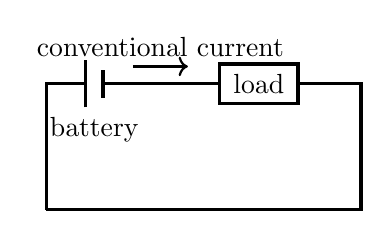
\begin{tikzpicture}[x=1cm,y=1cm]
\draw[very thick] (0,0)--(0,1.6)--(.5,1.6);
\draw[very thick] (.5,1.3)--(.5,1.9); \draw[very thick] (.72,1.42)--(.72,1.78);
\node[below] at (.61,1.3){battery};
\draw[very thick] (.72,1.6)--(2.2,1.6);
\draw[very thick] (2.2,1.35) rectangle (3.2,1.85);
\node at (2.7,1.6){load};
\draw[very thick] (3.2,1.6)--(4,1.6)--(4,0)--(0,0);
\draw[->,thick] (1.1,1.82)--(1.8,1.82) node[midway,above]{conventional current};
\end{tikzpicture}\end{center}}
\newcommand{\fielddiagram}{\begin{center}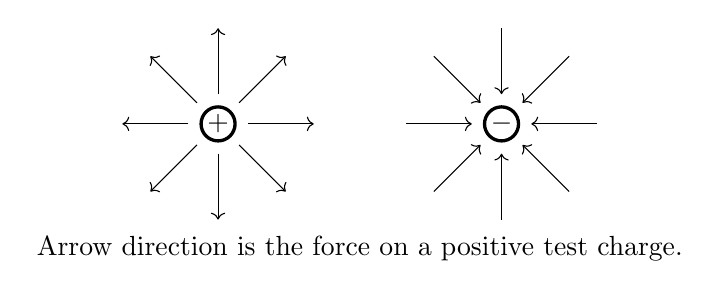
\begin{tikzpicture}[scale=.9]
\draw[very thick] (0,0) circle (.24); \node at (0,0){$+$};
\foreach \a in {0,45,...,315}{\draw[->] ({.42*cos(\a)},{.42*sin(\a)})--({1.35*cos(\a)},{1.35*sin(\a)});}
\draw[very thick] (4,0) circle (.24); \node at (4,0){$-$};
\foreach \a in {0,45,...,315}{\draw[<-] ({4+.42*cos(\a)},{.42*sin(\a)})--({4+1.35*cos(\a)},{1.35*sin(\a)});}
\node[below] at (2,-1.45){Arrow direction is the force on a positive test charge.};
\end{tikzpicture}\end{center}}
\newcommand{\coildiagram}{\begin{center}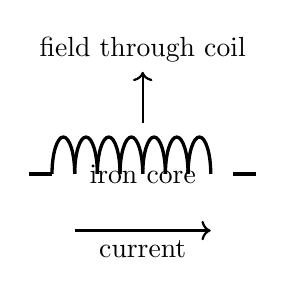
\begin{tikzpicture}[x=.72cm,y=.72cm]
\draw[very thick] (-2,0)--(-1.6,0);
\foreach \x in {-1.6,-1.2,...,1.2}{\draw[very thick] (\x,0) arc (180:0:.2 and .65);}
\draw[very thick] (1.6,0)--(2,0);
\draw[->,thick] (-1.2,-1)--(1.2,-1) node[midway,below]{current};
\draw[->,thick] (0,.9)--(0,1.8) node[above]{field through coil};
\node at (0,0){iron core};
\end{tikzpicture}\end{center}}
\newcommand{\inductiondiagram}{\begin{center}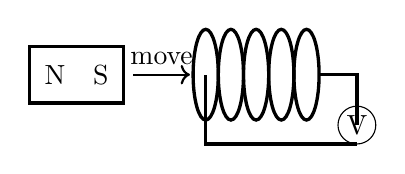
\begin{tikzpicture}[x=.8cm,y=.8cm]
\draw[very thick] (-2,-.45) rectangle (-.5,.45); \node at (-1.25,0){N\quad S};
\draw[->,thick] (-.35,0)--(.55,0) node[midway,above]{move};
\foreach \x in {.8,1.2,...,2.4}{\draw[very thick] (\x,0) ellipse (.2 and .72);}
\draw[very thick] (2.6,0)--(3.2,0)--(3.2,-.8);
\draw (3.2,-.8) circle (.3); \node at (3.2,-.8){V};
\draw[very thick] (3.2,-1.1)--(.8,-1.1)--(.8,0);
\end{tikzpicture}\end{center}}

\telosmeta{Electricity \& Magnetism}{\doctitle}{\docsubtitle}{20260726.001}
\begin{document}
\telosmasthead[\editiontag\ --- \docstrap]
\rolecard
\begin{materials}\materialslist\end{materials}
\begin{predict}\prediction\end{predict}
\diagram
\section{Investigate}
\procedure
\section{Explain from the evidence}
\explanation
\section{Change one thing}
\extension
\begin{recordbox}\end{recordbox}
\sourcefoot
\end{document}

